\documentclass[12pt]{article}
\usepackage[margin=1in]{geometry}
\usepackage{amsmath,amsthm,amssymb,scrextend}
\usepackage{pgfplots}
\pgfplotsset{compat=1.18}
\setlength{\parindent}{0pt}
\begin{document}
\newcommand{\ds}{\displaystyle}

\textbf{(i)(a)} Since Both sides are non-negative, squaring preserves the inequality

$$4x^2-8x+64\leq x^2+16x+64$$

$$3x^2-24x\leq0\implies 3x(x-8)\leq0$$

$$\boxed{0\leq x\leq8}$$

\bigskip\hrule\bigskip

\textbf{(i)(b)}

$$4x^2-8x+64\leq 9x^2-48x+64$$

$$5x^2-40x\geq0\implies 5x(x-8)\geq0$$

$$\boxed{x\leq0\ \text{ or }\ x\geq8}$$

\bigskip\hrule\bigskip

\textbf{(ii)(a)}

\begin{align*}
\left(\sqrt{4x^2-8x+64}+2(x-1)\right)\mathrm{f}(x)
&=\left(4x^2-8x+64\right)-4(x-1)^2\\
&=\left(4x^2-8x+64\right)-\left(4x^2-8x+4\right)\\
&=60
\end{align*}

$$\mathrm{f}(x)=\frac{60}{\sqrt{4x^2-8x+64}+2(x-1)}$$

As $\ds x\to\infty$, the denominator $\to\infty$

$$\implies \boxed{\mathrm{f}(x)\to0}$$

\bigskip\hrule\bigskip

\textbf{(ii)(b)}

$$y=\sqrt{4x^2-8x+64}=2\sqrt{(x-1)^2+15}$$

$$\frac{y^2}{60}-\frac{(x-1)^2}{15}=1,\qquad y>0$$

Minimum point $\ds \left(1,2\sqrt{15}\right)$, $\ds y$-intercept $8$, asymptotes $\ds y=\pm2(x-1)$

$$\mathrm{f}(x)>0\implies \sqrt{4x^2-8x+64}>2(x-1)\ \text{ for all }x$$

\begin{center}
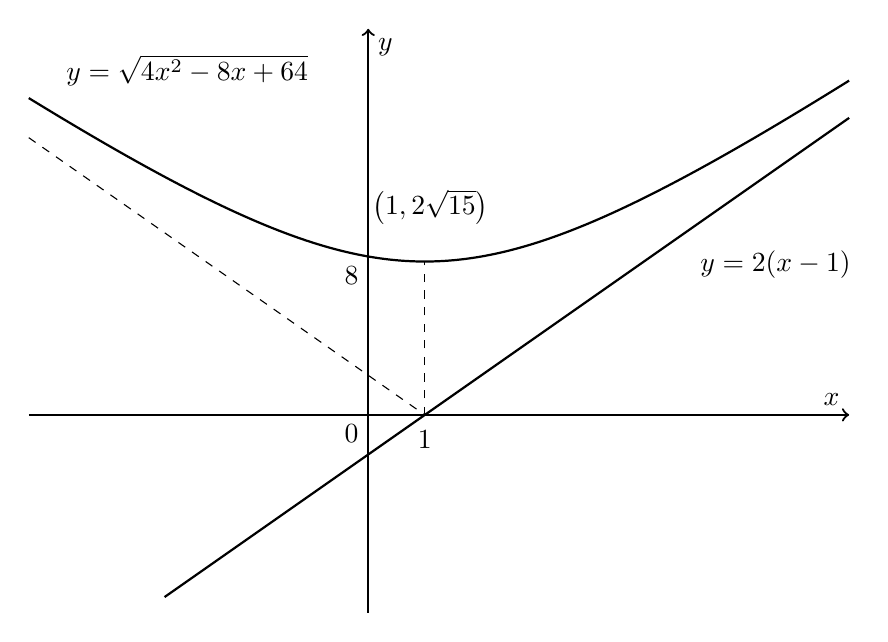
\begin{tikzpicture}
\begin{axis}[
    axis lines=middle,
    xmin=-6, xmax=8.5,
    ymin=-10, ymax=19.5,
    width=12cm,
    height=9cm,
    axis line style={->, thick},
    xlabel={$x$},
    ylabel={$y$},
    xtick={1},
    ytick=\empty,
    tick style={draw=none},
    clip=false,
    samples=200
]
\addplot[domain=-6:8.5, thick] {2*sqrt((x-1)^2+15)};
\addplot[domain=-3.6:8.5, thick] {2*(x-1)};
\addplot[dashed, domain=-6:1] {-2*(x-1)};
\addplot[dashed] coordinates {(1,0) (1,7.746)};
\node at (axis cs:0,0) [below left] {$0$};
\node at (axis cs:0,8) [below left] {$8$};
\node at (axis cs:1.1,10.5) {$\left(1,2\sqrt{15}\right)$};
\node at (axis cs:-3.2,17.4) {$y=\sqrt{4x^2-8x+64}$};
\node at (axis cs:7.2,7.6) {$y=2(x-1)$};
\end{axis}
\end{tikzpicture}
\end{center}

\bigskip\hrule\bigskip

\textbf{(iii)}

$$4x^2-5x+4=4\left(x-\frac58\right)^2+\frac{39}{16}>0$$

$$4x^2-5x+4\leq m^2x^2+2mcx+c^2$$

$$\left(m^2-4\right)x^2+(2mc+5)x+c^2-4\geq0$$

The solution set $\{x:x\geq3\}$ is a half-line, so the quadratic term must vanish.

$$m^2-4=0\implies m=\pm2$$

Take $\ds m=2$:

$$(4c+5)x+c^2-4\geq0$$

$$4c+5>0\quad\text{and}\quad c^2-4=-3(4c+5)$$

$$c^2+12c+11=0\implies (c+1)(c+11)=0\implies c=-1,\ -11$$

$$c=-11\implies 4c+5=-39<0\text{ (rejected)}$$

$$\boxed{m=2,\quad c=-1}$$

Check:
$$4x^2-5x+4\leq(2x-1)^2=4x^2-4x+1\implies x\geq3$$

\bigskip\hrule\bigskip

\textbf{(iv)}

$$\left|x^2+px+q\right|\leq mx+c
\iff -(mx+c)\leq x^2+px+q\leq mx+c$$

$$x^2+(p-m)x+(q-c)\leq0\qquad\text{and}\qquad x^2+(p+m)x+(q+c)\geq0$$

The first gives a closed interval $[\alpha,\beta]$, the second gives everything outside an open interval $(\gamma,\delta)$.

$$\{-5\leq x\leq1\}\cup\{5\leq x\leq7\}=[-5,7]\setminus(1,5)$$

$$\implies \alpha=-5,\ \beta=7,\ \gamma=1,\ \delta=5$$

$$x^2+(p-m)x+(q-c)=(x+5)(x-7)=x^2-2x-35$$

$$x^2+(p+m)x+(q+c)=(x-1)(x-5)=x^2-6x+5$$


$$
\begin{cases}
p-m=-2 &\\
p+m=-6 &
\end{cases}
\implies
\begin{cases}
p=-4 &\\
m=-2 &
\end{cases}
$$

$$
\begin{cases}
q-c=-35 &\\
q+c=-5 &
\end{cases}
\implies
\begin{cases}
q=-15 &\\
c=-20 &
\end{cases}
$$

$$\text{Since }\left|x^2+px+q\right|\geq 0,\  mx+c=20-2x\geq0\text{ on }-5\leq x\leq7$$

\bigskip
\hrule
\begin{center}
    This solution was submitted by \textbf{Jon}\\[4pt]
    Published and refined by \textbf{Jon}\\[8pt]
    \textit{Last updated: September 5, 2026}
\end{center}

\end{document}
